\documentclass[10pt]{article}

% One shared preamble: portrait front matter/figures; landscape tables.
\usepackage[a4paper,margin=20mm]{geometry}
% Shared style for the supplementary tables. No figure dependencies.
% Page geometry is controlled by supplementary_information.tex.
\usepackage[T1]{fontenc}
\usepackage{lmodern,amsmath,booktabs,longtable,array}
\usepackage{caption}
\usepackage[hidelinks]{hyperref}
\usepackage{microtype}
\newcolumntype{L}[1]{>{\raggedright\arraybackslash}p{#1}}
\newcolumntype{C}[1]{>{\centering\arraybackslash}p{#1}}
\newcolumntype{R}[1]{>{\raggedleft\arraybackslash}p{#1}}
\newlength{\ABMtablewidth}
% Same-line estimate [95% interval], with mathematical minus signs.
\newcommand{\ABMci}[3]{\mbox{\ensuremath{#1}\,{\fontsize{8}{10}\selectfont\ensuremath{[#2,\,#3]}}}}
\newcommand{\ABMnote}[1]{{\fontsize{8.5}{11}\selectfont\raggedright\textit{Note.} #1\par}}
\renewcommand{\thetable}{S\arabic{table}}
\renewcommand{\listtablename}{List of tables}
\captionsetup[table]{font=small,labelfont=bf,labelsep=space,justification=raggedright,singlelinecheck=false,skip=6pt}
\setlength{\LTpre}{0pt}
\setlength{\LTpost}{0pt}
\setlength{\LTleft}{\fill}
\setlength{\LTright}{\fill}
\setlength{\parindent}{0pt}
\setlength{\parskip}{5pt}
\setlength{\emergencystretch}{2em}
\pagestyle{plain}

\usepackage{graphicx,pdflscape,eso-pic}
\newcommand{\ABMArticleTitle}{%
Dynamic Evaluation of Governance Strategies for Mitigating
Social Media Data Pollution: An Agent-Based Modeling Approach}

\newcommand{\ABMJournal}{Complex \& Intelligent Systems}

\newcommand{\ABMAuthors}{%
Jingyu Lin, Qingxing Zeng, Kai Liu, and Han Huang}

\newcommand{\ABMCorrespondingAffiliation}{%
School of Law, South China University of Technology,
Zhonghuan Road East, Guangzhou 510006, Guangdong, China}

\newcommand{\ABMCorrespondingEmail}{%
Qingxing Zeng: \texttt{qxzeng@scut.edu.cn}}

\newcommand{\ABMEmpty}{}
\renewcommand{\thefigure}{S\arabic{figure}}
\captionsetup[figure]{font=small,labelfont=bf,labelsep=colon,
  justification=justified,singlelinecheck=false,skip=8pt}
\hypersetup{pdftitle={Supplementary Information},bookmarksnumbered=true,pdfview=Fit,pdfstartview=Fit}
\setcounter{tocdepth}{2}
\setcounter{secnumdepth}{1}
\makeatletter
% Wide enough for both "Table S17" and "Fig. S11" in the unified contents.
\renewcommand{\l@subsection}{\@dottedtocline{2}{1.5em}{5.5em}}
\makeatother

% Each table is a longtable, so its TOC anchor is placed on its first page.
\newcommand{\ABMInputTable}[3]{%
  \clearpage
  \phantomsection
  \addcontentsline{toc}{subsection}{\protect\numberline{Table~#2}#3}%
  \input{#1}%
}

% Keep the folio horizontal and centred at the bottom of landscape pages.
\newif\ifABMLandscapePage
\AddToShipoutPictureFG{%
  \ifABMLandscapePage
    \AtPageLowerLeft{%
      \put(\LenToUnit{\dimexpr\paperwidth-8mm\relax},\LenToUnit{0.5\paperheight}){%
        \rotatebox{90}{\makebox[0pt]{\normalfont\normalsize\thepage}}}%
    }%
  \fi
}

\begin{document}
\begin{center}
{\LARGE\bfseries Supplementary Information}\\[5pt]
{\large Tables S1--S17 and Figures S1--S11}
\end{center}
\ifx\ABMArticleTitle\ABMEmpty\else
\begin{center}
  \begin{minipage}{0.90\textwidth}
    \centering
    \fontsize{13}{17}\selectfont
    \bfseries
    \ABMArticleTitle\par
  \end{minipage}
\end{center}
\vspace{3pt}
\fi
\ifx\ABMJournal\ABMEmpty\else\textbf{Journal:} \ABMJournal\par\fi
\ifx\ABMAuthors\ABMEmpty\else\textbf{Authors:} \ABMAuthors\par\fi
\ifx\ABMCorrespondingAffiliation\ABMEmpty\else\textbf{Corresponding author affiliation:} \ABMCorrespondingAffiliation\par\fi
\ifx\ABMCorrespondingEmail\ABMEmpty\else\textbf{Correspondence:} \ABMCorrespondingEmail\par\fi
\begingroup
\small
\setlength{\parskip}{0pt}
\tableofcontents
\endgroup
\clearpage

\section{Supplementary tables}\label{sec:supp-tables}
\subsection*{Reading the tables}

Tables S1--S8 report condition summaries; Tables S9--S17 report prespecified comparisons. Estimates and their 95\% intervals appear together, except in Table S10, which uses separate interval columns. Each condition uses 30 independent runs; repeated appearances of an identical condition reuse the same runs.

Condition summaries use Student-$t$ confidence intervals. Comparisons use marginal, unadjusted Welch intervals, except for Table S10: its dimensionless PAWN-index differences have separate row-bootstrap stability and within-point Monte Carlo intervals, based on 500 LHS points per regime and initial pollution level, with 30 runs per point. These two interval types are not combined.

Outcome levels are percentages and their differences are percentage points unless stated otherwise. Network diagnostics and review burdens are counts; review totals include repeated reviews. Table notes specify subtraction order, units, valid sample sizes and exceptions. Unrounded values and identifiers are retained in the accompanying CSV files.

\clearpage
\newgeometry{margin=15mm}
\ABMLandscapePagetrue\pagestyle{empty}
\begin{landscape}
\ABMInputTable{tables/tableS_network.tex}{S1}{Realized network diagnostics}
\ABMInputTable{tables/tableS1_P3.tex}{S2}{Outcomes under fixed and state-responsive platform moderation}
\ABMInputTable{tables/tableS1_P3_workload.tex}{S3}{Review burden under fixed and state-responsive platform moderation}
\ABMInputTable{tables/tableS3_P5_legal.tex}{S4}{Legal outcomes under random and degree-targeted selection}
\ABMInputTable{tables/tableS3_P5_platform.tex}{S5}{Platform outcomes under random and degree-targeted selection}
\ABMInputTable{tables/tableS4_P6_legal.tex}{S6}{Legal outcomes across true-positive and true-negative rates}
\ABMInputTable{tables/tableS4_P6_platform50.tex}{S7}{Platform outcomes across true-positive and true-negative rates at 50\% coverage}
\ABMInputTable{tables/tableS4_P6_platform75.tex}{S8}{Platform outcomes across true-positive and true-negative rates at 75\% coverage}
\ABMInputTable{tables/tableS9_H1.tex}{S9}{H1: differences in mean-effectiveness gains}
\ABMInputTable{tables/tableS10_H2.tex}{S10}{H2: PAWN index differences and wrongful-exposure comparisons}
\ABMInputTable{tables/tableS11_H3.tex}{S11}{H3: effectiveness and wrongful-exposure changes}
\ABMInputTable{tables/tableS12_P3_differences.tex}{S12}{Outcome differences: state-responsive minus fixed moderation}
\ABMInputTable{tables/tableS13_P5_differences.tex}{S13}{Outcome differences: degree-targeted minus random selection}
\ABMInputTable{tables/tableS14_P6_differences.tex}{S14}{Outcome differences from separately increasing TPR and TNR}
\ABMInputTable{tables/tableS15_topology_differences.tex}{S15}{Network-topology differences relative to BA}
\ABMInputTable{tables/tableS16_scale_differences.tex}{S16}{Network-size differences: 5,000 minus 1,000 nodes}
\ABMInputTable{tables/tableS17_P3_workload_differences.tex}{S17}{Review-burden differences: state-responsive minus fixed moderation}

\end{landscape}
\ABMLandscapePagefalse\pagestyle{plain}
\restoregeometry
\clearpage

\section{Supplementary figures}\label{sec:supp-figures}
\subsection*{Reading the figures}

Mean effectiveness $\bar E$ averages steps 1--50 within each run. Wrongful exposure $O(50)$ is the percentage of distinct accounts ever wronged by step 50; removal precision $P_R(50)$ averages defined run-level ratios. Review totals count events, including repeated reviews of the same account. Figure S1 expresses review totals in thousands.

Figures S1--S4 summarise 30 independent runs per condition. Figures S5--S11 use 500 Latin hypercube sampling (LHS) points per governance regime and initial pollution level, with 30 runs per point. The same responses are reused across diagnostics and input--response panels.

Displayed 95\% intervals are marginal, unadjusted and not clipped. Row-bootstrap intervals describe stability under design-point resampling; within-point Monte Carlo intervals describe simulation uncertainty at fixed parameter points. These separate bootstrap intervals are not combined and need not contain the point estimate.

Input--response lines connect descriptive bin means. Continuous inputs use fixed empirical-quantile bins from the full LHS design; legal response intervals use the pairs 1--2, 3--4, \ldots, 19--20 steps. Full values and identifiers remain in the CSV files.

\clearpage
\begin{figure}[p]
\centering
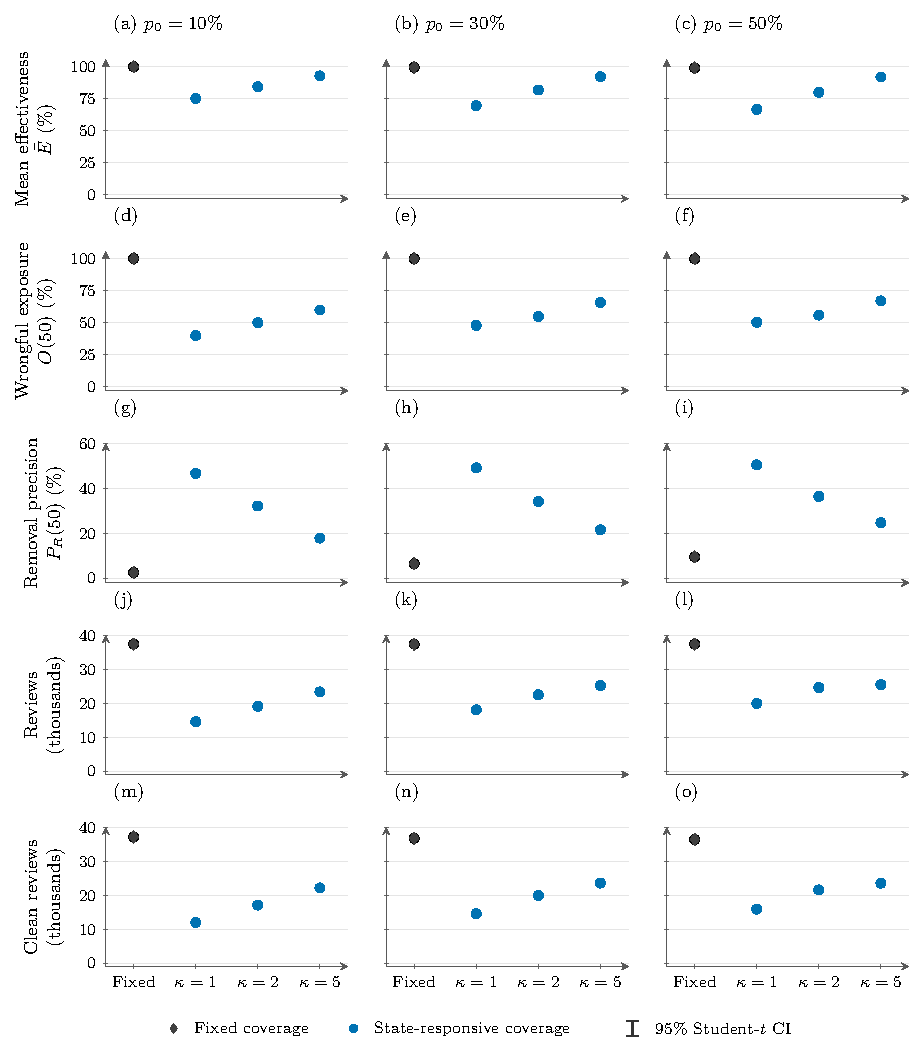
\includegraphics[width=\textwidth,height=0.78\textheight,keepaspectratio]{figures/figS1_workload.pdf}
\caption{Platform workload specifications (P3). Fixed auditing reviews 75\% of accounts per step; responsive auditing uses $\min\{N,\operatorname{round}(0.75N),\operatorname{round}(\kappa I_t)\}$, where $I_t$ is the number of polluted accounts before review and $\kappa=1,2,5$. Both modes use TPR$=$TNR$=80\%$. Points and whiskers show means and 95\% Student-$t$ CIs. Precision is defined in all 30 runs per condition; review counts are in thousands.}
\label{fig:supp-figS1_workload}
\addcontentsline{toc}{subsection}{\protect\numberline{Fig.~\thefigure}Fixed and state-responsive platform auditing}
\end{figure}
\clearpage

\begin{figure}[p]
\centering
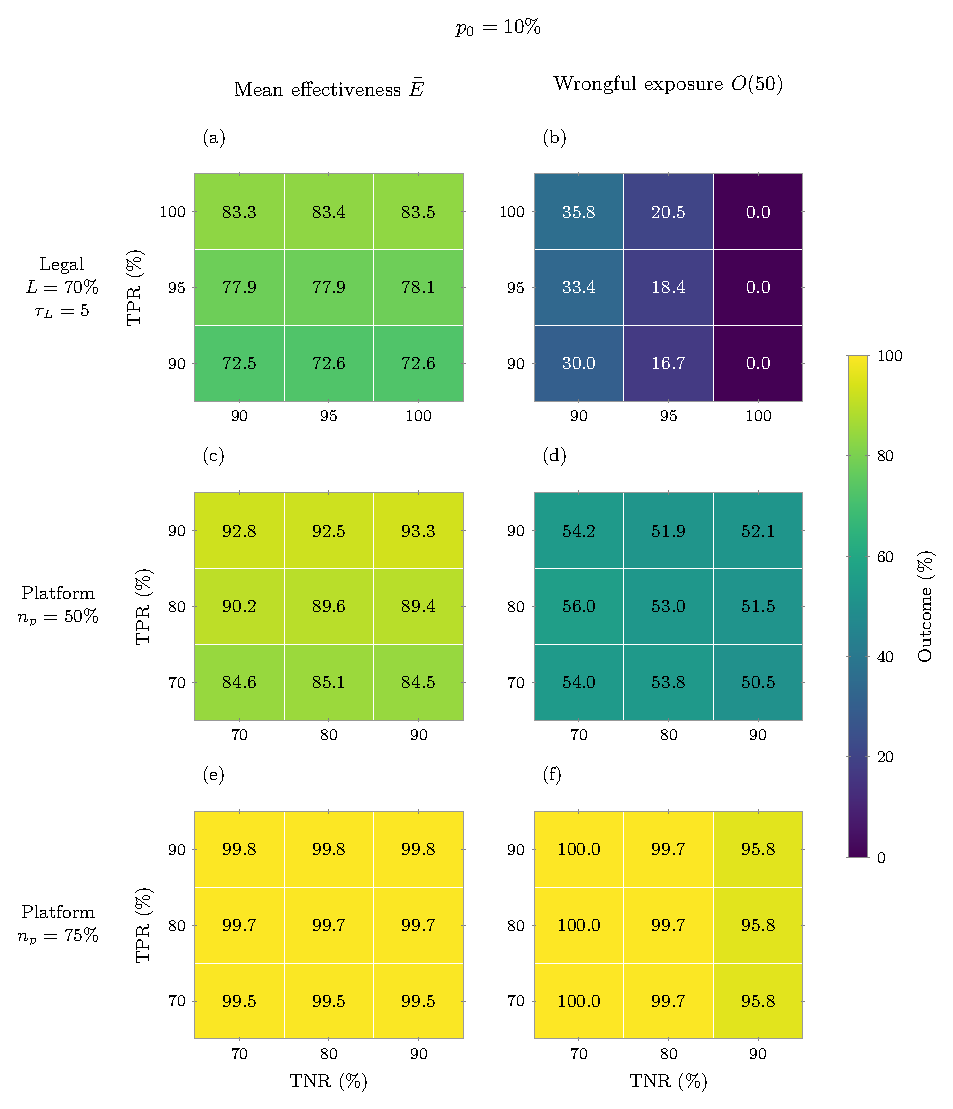
\includegraphics[width=\textwidth,height=0.78\textheight,keepaspectratio]{figures/figS4_accuracy_p10.pdf}
\caption{Independent TPR and TNR variation (P6), $p_0=10\%$. Rows identify governance and coverage settings; platform auditing is fixed. Cells show 30-run means, rounded to one decimal, on a common 0--100\% scale. Full means and 95\% Student-$t$ CIs are retained in the plot CSVs. False-positive flags accumulate wrongful exposure without deleting accounts or links or feeding back into diffusion.}
\label{fig:supp-figS4_accuracy_p10}
\addcontentsline{toc}{subsection}{\protect\numberline{Fig.~\thefigure}Independent TPR/TNR variation: \texorpdfstring{$p_0=10\%$}{p0=10\%}}
\end{figure}
\clearpage

\begin{figure}[p]
\centering
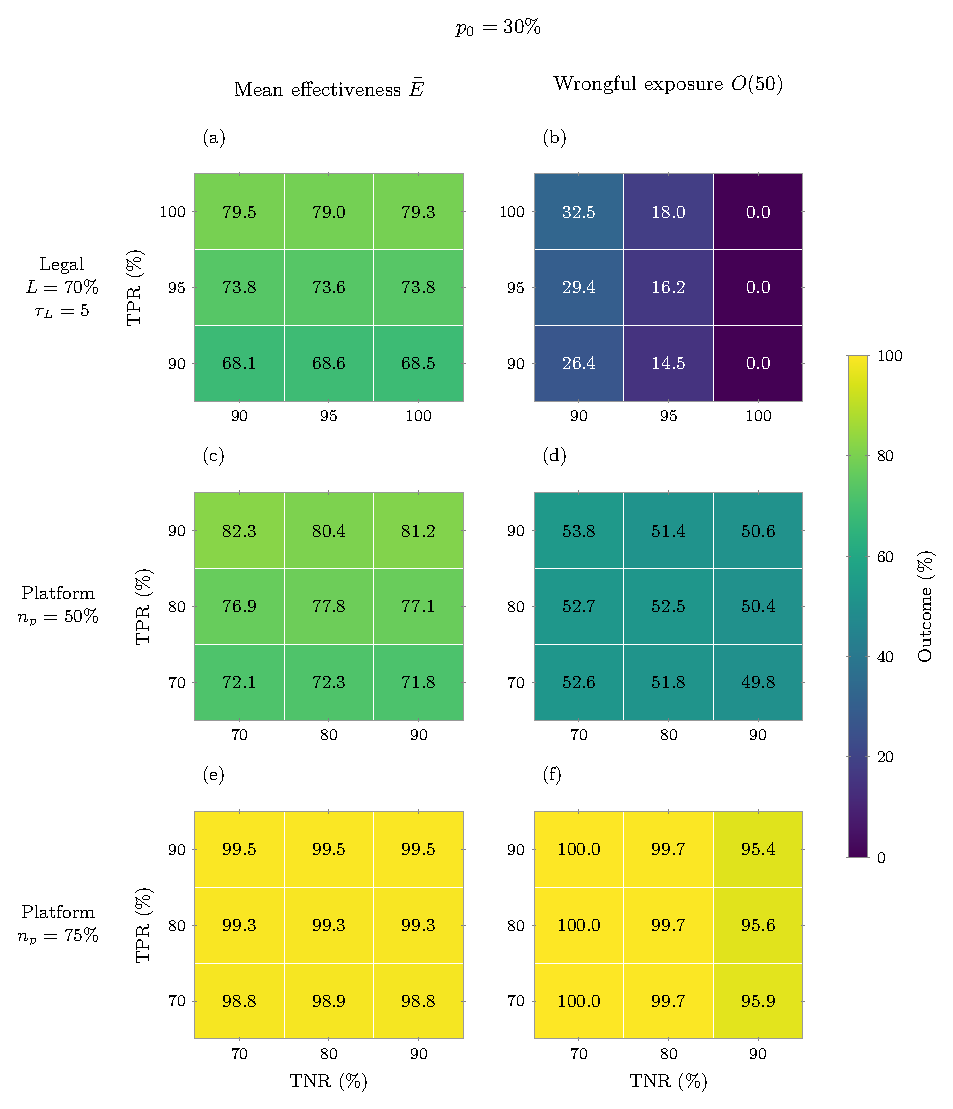
\includegraphics[width=\textwidth,height=0.78\textheight,keepaspectratio]{figures/figS4_accuracy_p30.pdf}
\caption{Independent TPR and TNR variation at $p_0=30\%$. Design, cell summaries and colour scale follow Fig.~\ref{fig:supp-figS4_accuracy_p10}.}
\label{fig:supp-figS4_accuracy_p30}
\addcontentsline{toc}{subsection}{\protect\numberline{Fig.~\thefigure}Independent TPR/TNR variation: \texorpdfstring{$p_0=30\%$}{p0=30\%}}
\end{figure}
\clearpage

\begin{figure}[p]
\centering
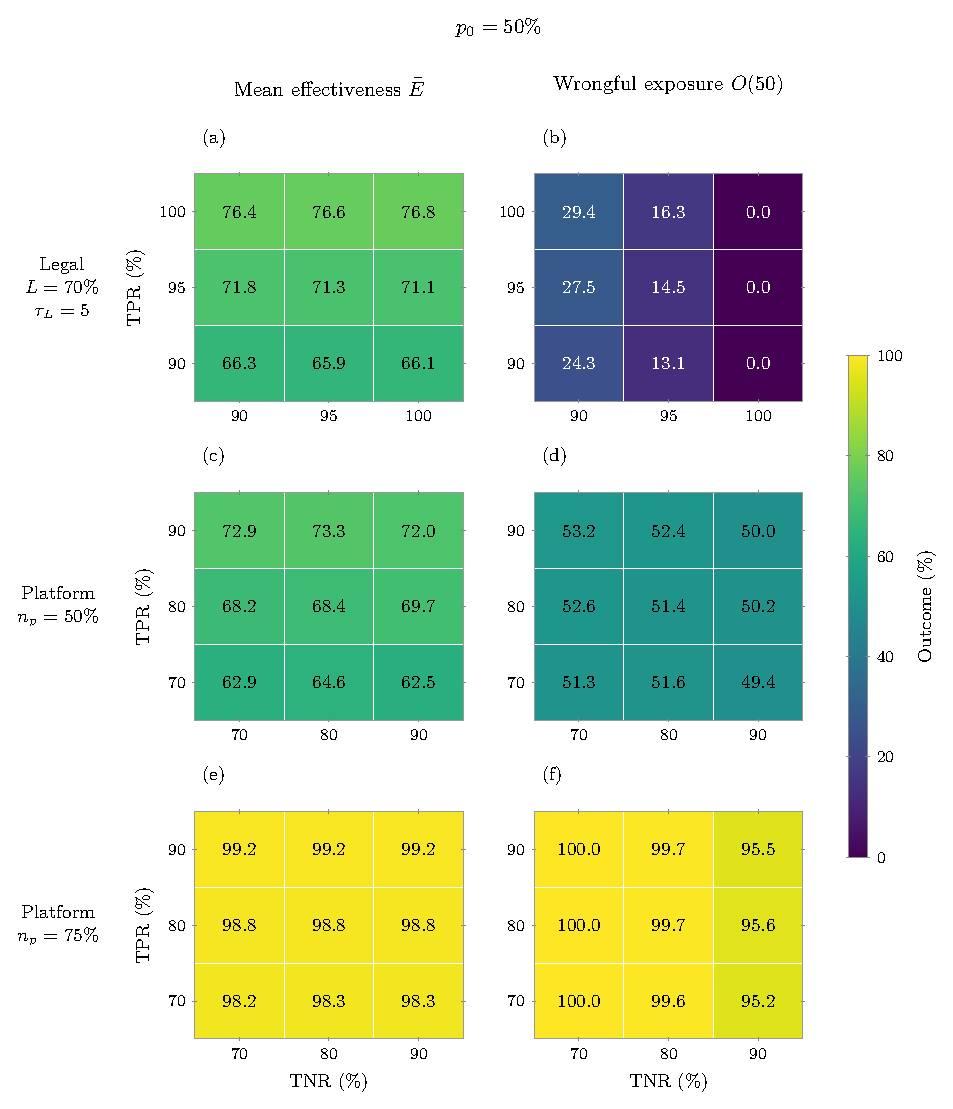
\includegraphics[width=\textwidth,height=0.78\textheight,keepaspectratio]{figures/figS4_accuracy_p50.pdf}
\caption{Independent TPR and TNR variation at $p_0=50\%$. Design, cell summaries and colour scale follow Fig.~\ref{fig:supp-figS4_accuracy_p10}.}
\label{fig:supp-figS4_accuracy_p50}
\addcontentsline{toc}{subsection}{\protect\numberline{Fig.~\thefigure}Independent TPR/TNR variation: \texorpdfstring{$p_0=50\%$}{p0=50\%}}
\end{figure}
\clearpage

\begin{figure}[p]
\centering
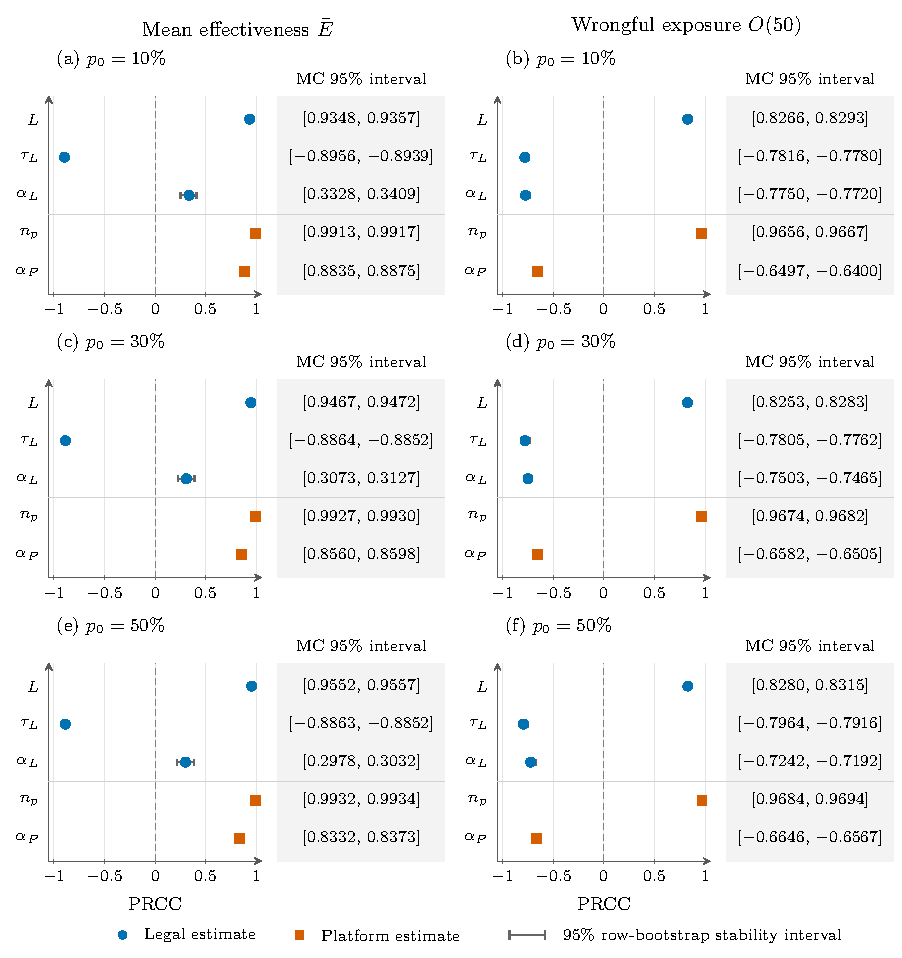
\includegraphics[width=\textwidth,height=0.78\textheight,keepaspectratio]{figures/figS2b_PRCC.pdf}
\caption{Partial rank correlations (PRCC). Points and whiskers show estimates and marginal 95\% row-bootstrap stability intervals; shaded columns report separate 95\% within-point Monte Carlo intervals. Each bootstrap uses 1,000 resamples. Row resampling does not preserve LHS strata. PRCC describes conditional rank association; directional interpretation relies on monotonicity and does not replace the primary PAWN analysis.}
\label{fig:supp-figS2b_PRCC}
\addcontentsline{toc}{subsection}{\protect\numberline{Fig.~\thefigure}PRCC estimates and uncertainty intervals}
\end{figure}
\clearpage

\begin{figure}[p]
\centering
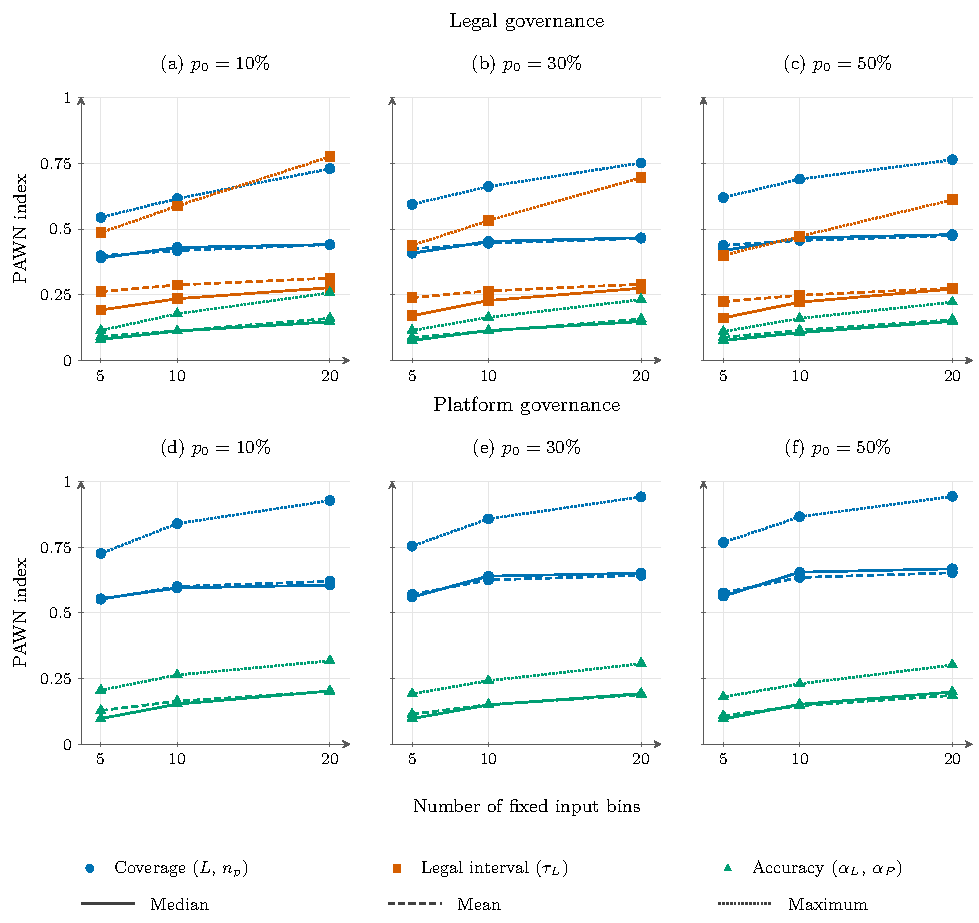
\includegraphics[width=\textwidth,height=0.78\textheight,keepaspectratio]{figures/figS2d_bins_E_mean.pdf}
\caption{PAWN diagnostics for mean effectiveness $\bar E$. Point estimates compare 5, 10 and 20 fixed input bins with median, mean and maximum aggregation; the primary estimator remains the 10-bin median. Full bootstrap intervals, 20- versus 30-run estimates and rankings are provided in \texttt{sensitivity\_diagnostics.csv}.}
\label{fig:supp-figS2d_bins_E_mean}
\addcontentsline{toc}{subsection}{\protect\numberline{Fig.~\thefigure}PAWN diagnostics: mean effectiveness}
\end{figure}
\clearpage

\begin{figure}[p]
\centering
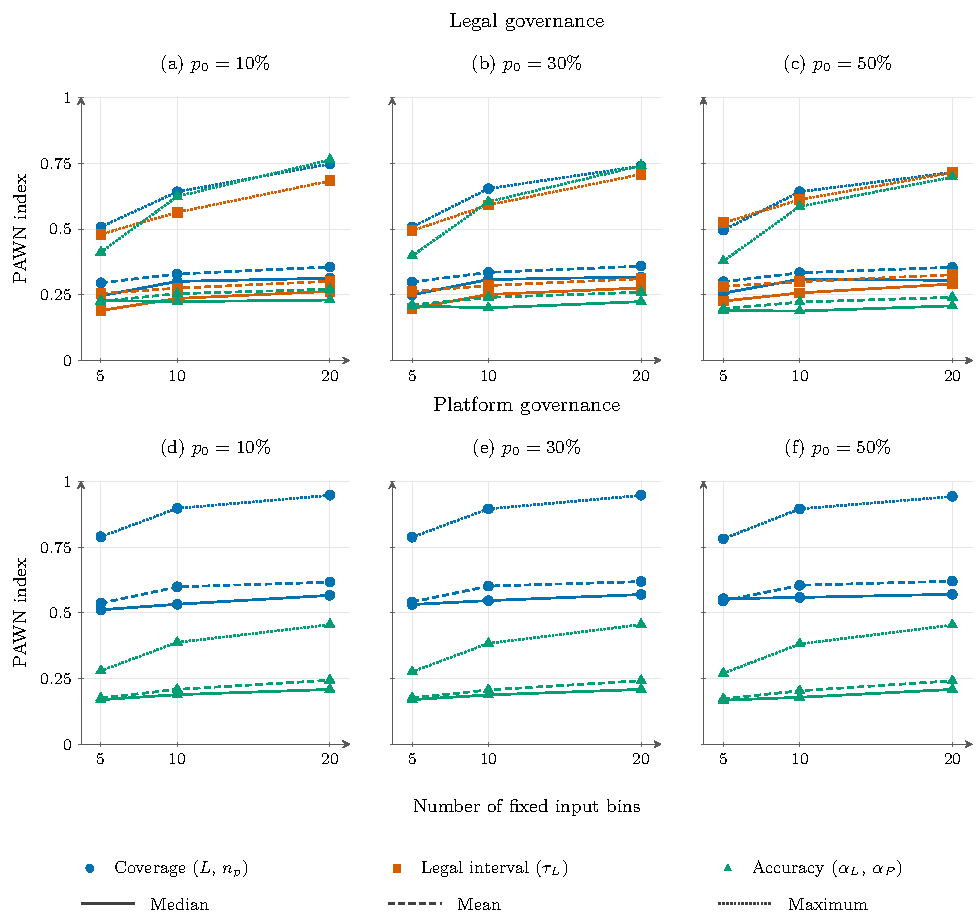
\includegraphics[width=\textwidth,height=0.78\textheight,keepaspectratio]{figures/figS2d_bins_O_final.pdf}
\caption{PAWN diagnostics for wrongful exposure $O(50)$. Settings and graphical encodings follow Fig.~\ref{fig:supp-figS2d_bins_E_mean}.}
\label{fig:supp-figS2d_bins_O_final}
\addcontentsline{toc}{subsection}{\protect\numberline{Fig.~\thefigure}PAWN diagnostics: wrongful exposure}
\end{figure}
\clearpage

\begin{figure}[p]
\centering
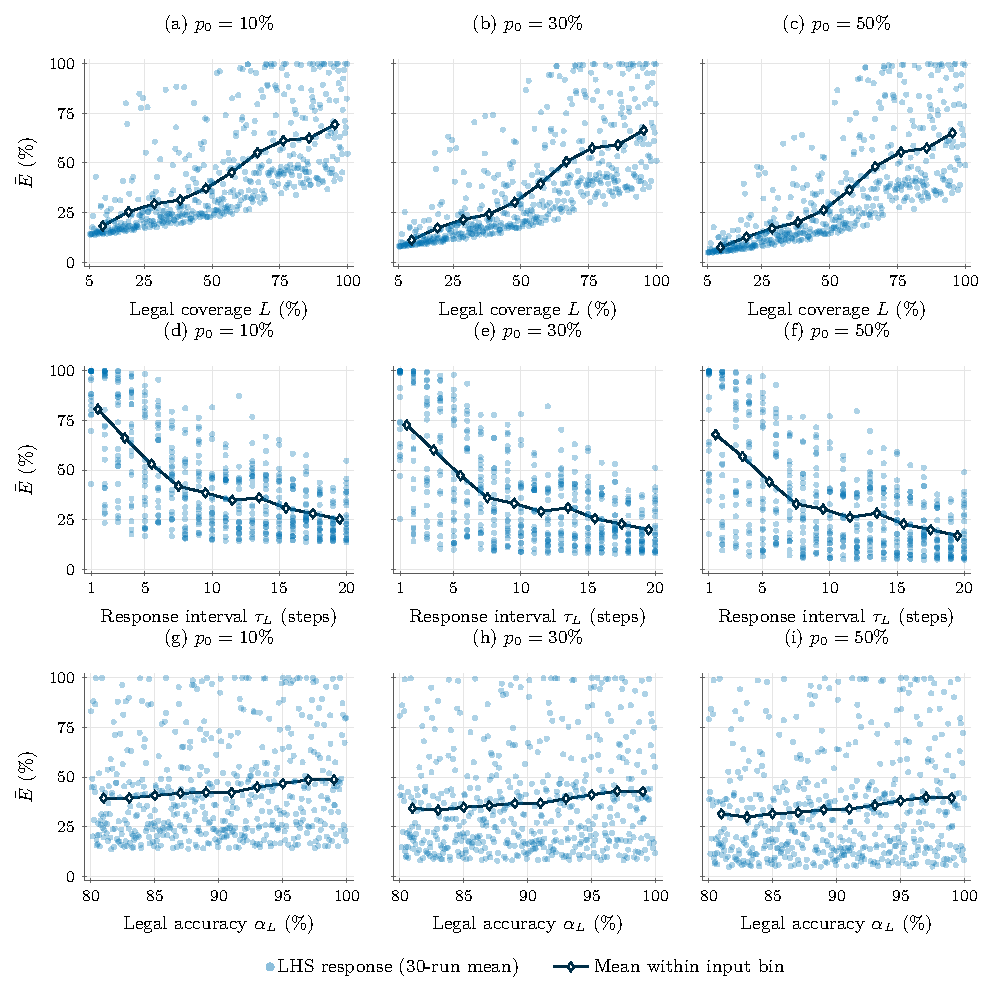
\includegraphics[width=\textwidth,height=0.78\textheight,keepaspectratio]{figures/sensitivity_response_legal_E_mean.pdf}
\caption{Input--response patterns for legal governance and mean effectiveness $\bar E$. Each panel shows 500 LHS responses, each averaged over 30 runs; other inputs vary simultaneously. Lines connect means within 10 fixed input bins. These descriptive summaries are neither isolated single-input causal curves nor confidence bands; they help assess saturation, discreteness and monotonicity.}
\label{fig:supp-sensitivity_response_legal_E_mean}
\addcontentsline{toc}{subsection}{\protect\numberline{Fig.~\thefigure}Legal input--response patterns: mean effectiveness}
\end{figure}
\clearpage

\begin{figure}[p]
\centering
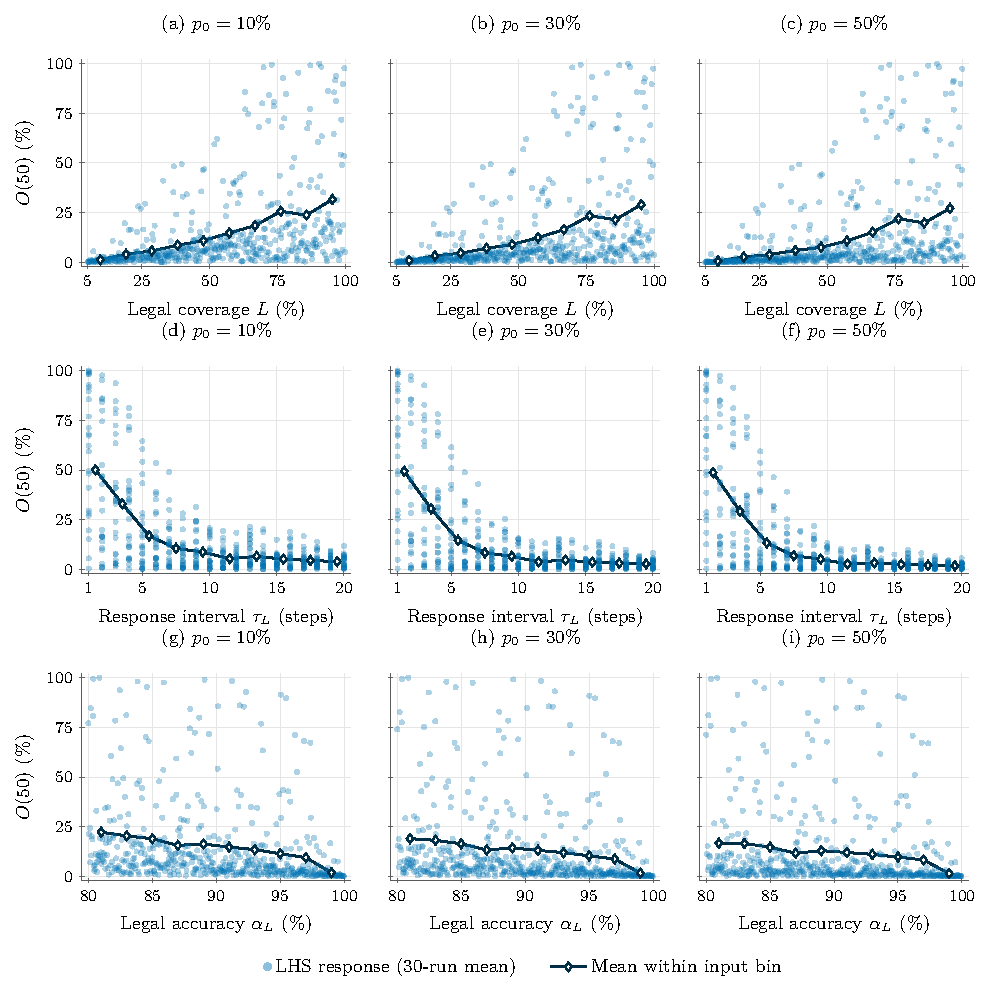
\includegraphics[width=\textwidth,height=0.78\textheight,keepaspectratio]{figures/sensitivity_response_legal_O_final.pdf}
\caption{Input--response patterns for legal governance and wrongful exposure $O(50)$. Sampling, bin summaries and interpretation follow Fig.~\ref{fig:supp-sensitivity_response_legal_E_mean}.}
\label{fig:supp-sensitivity_response_legal_O_final}
\addcontentsline{toc}{subsection}{\protect\numberline{Fig.~\thefigure}Legal input--response patterns: wrongful exposure}
\end{figure}
\clearpage

\begin{figure}[p]
\centering
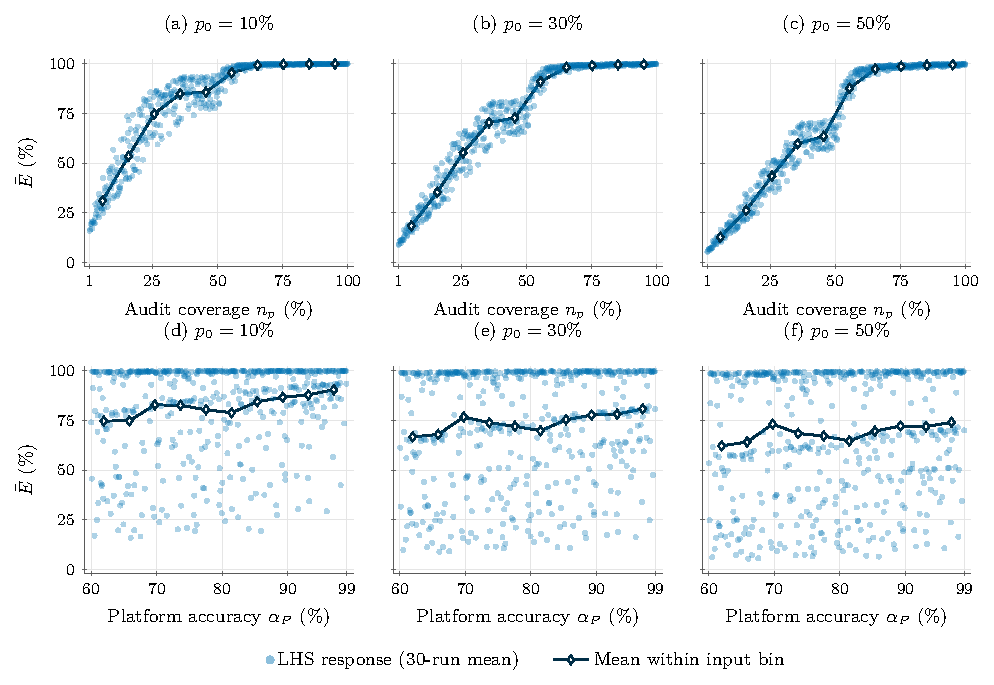
\includegraphics[width=\textwidth,height=0.78\textheight,keepaspectratio]{figures/sensitivity_response_platform_E_mean.pdf}
\caption{Input--response patterns for platform governance and mean effectiveness $\bar E$. Sampling, bin summaries and interpretation follow Fig.~\ref{fig:supp-sensitivity_response_legal_E_mean}.}
\label{fig:supp-sensitivity_response_platform_E_mean}
\addcontentsline{toc}{subsection}{\protect\numberline{Fig.~\thefigure}Platform input--response patterns: mean effectiveness}
\end{figure}
\clearpage

\begin{figure}[p]
\centering
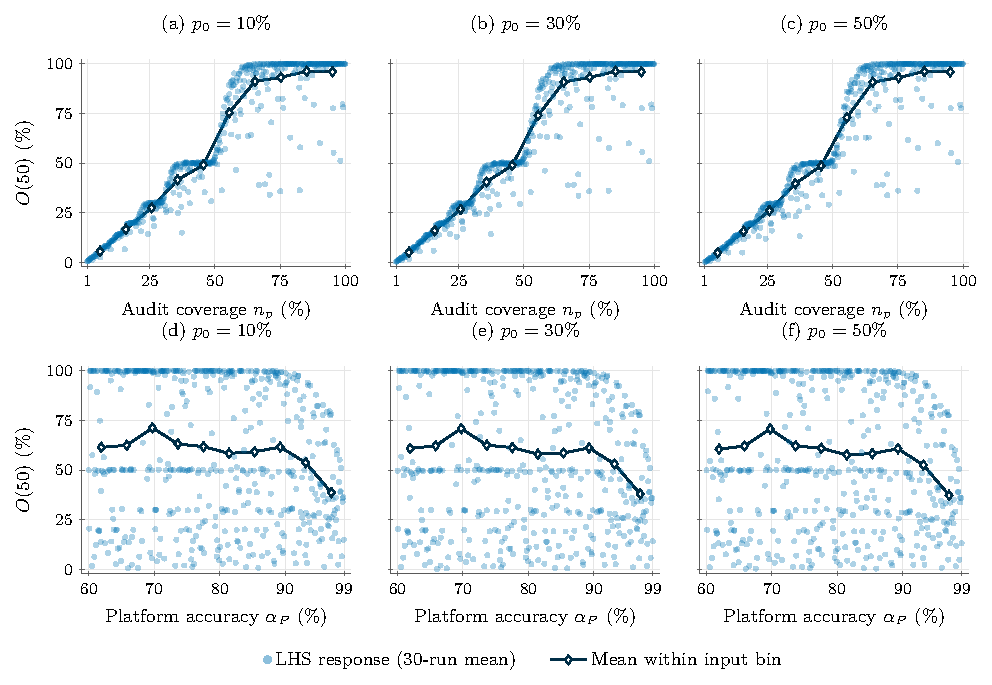
\includegraphics[width=\textwidth,height=0.78\textheight,keepaspectratio]{figures/sensitivity_response_platform_O_final.pdf}
\caption{Input--response patterns for platform governance and wrongful exposure $O(50)$. Sampling, bin summaries and interpretation follow Fig.~\ref{fig:supp-sensitivity_response_legal_E_mean}.}
\label{fig:supp-sensitivity_response_platform_O_final}
\addcontentsline{toc}{subsection}{\protect\numberline{Fig.~\thefigure}Platform input--response patterns: wrongful exposure}
\end{figure}
\clearpage

\end{document}
